\chapter{Conclusions and Future Directions}
\label{chap:chapter5}
\section{Chapter \ref{chap:chapter2} - Multi-state design and polyspecificity}
I expound on the limitations of \rosettadesign by looking at the imperfect agreement between what we expect \rosettadesign to recovery and what was actually observed. I bin these into three categories, Mature sequence bias, evolutionary sequence bias, and incomplete ensemble bias. Section \ref{sec:maturebias} accounts for mature sequence bias, which may be the most difficult to expand understand. When a residue is ``important'' for most of the antibody-antigen complexes, it should be recovered often. However if it only is important in a few complexes, then any given residue can meet the design challenges for the complexes in which it is not important.

Section \ref{sec:evobias} refers to evolutionary sequence bias. Here we may see imperfect agreement with the design and actual antibody sequence simply because the antibody has not achieved maximal potency. \rosettadesign may have selected better amino acid sequences for the epitope. Give enough time to for complete antibody evolution, the sequence may have matched. This is founded on the principle that \rosettadesign gives the best sequence for any design challenge.

Section \ref{sec:limits} gives the limits of computation including the finite ensemble size that states there are not enough PDBs to compensate for ``structural space'' that \rosettadesign samples. This section also details some of the more classic limitations including the limits of the \rosetta scoring function and limitations of the sampling algorithms. In the future this may be ameliorated with more structures being deposited to the PDB, and improvements to the scoring function including explicit solvent modeling.

The power of chapter \ref{chap:chapter2} is in the future directions. While we use multi-state design to interrogate the flexibility of the germline repertoire, the end goal was always to design cross-binding antibodies. Many pathogens which evade traditional vaccination do so by evolving multiple serotypes or antigenic variants that encompass a tremendous sequence space. HIV, Influenza and Dengue virus (DENV) are such examples of antibodies which use antigenic variation as a means to evade a broadly protective immunogenic response. It is to these pathogens that a broad cross-reactive response will be critical \citep{Corti:2013ex,Lanzavecchia:2009dd,Corti:2011ku,Simonelli:2013jc}. Multi-state design will be invaluable in the design of these antibodies. Consider \ref{fig:fig5_1}, here we take a known cross-reactive group 1 antibody against influenza known as CR6261 \citep{Throsby:2008dc} which does not bind to Influenza type B.

\begin{figure}[t]
   \centering
   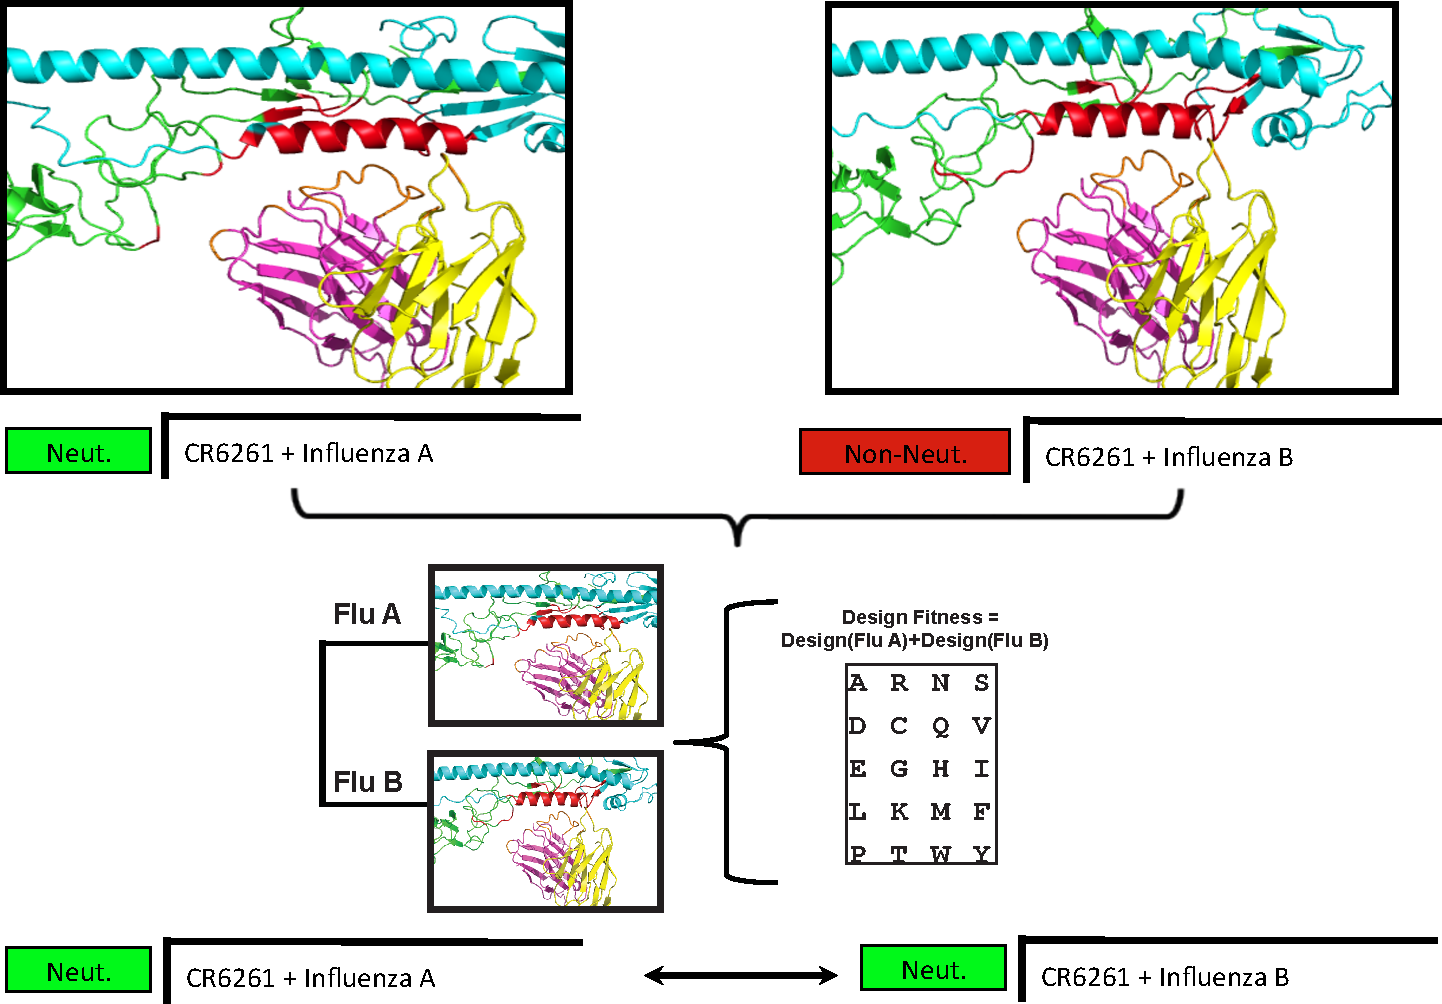
\includegraphics[width=.9\textwidth]{images/chapter5/figure5_1.pdf}
   \caption[Multi-state Design of Broadly Neutralizing Influenza Antibodies]{Multi-state design of broadly neutralizing influenza antibodies. Initially, the antibody CR6261 only binds and neutralizes only Influenza A subtypes. Using multi-state design I plan to make minimal mutations at the interface that allow binding to Influenza type B while retaining binding to Influenza type A. This principle allows me to design in cross-specificity.}
       \label{fig:fig5_1}
\end{figure}


I even took this idea into the lab looking at special cases for influenza antibody. I considered the antibody CR6261 as it was bound to the stem portion of influenza \citep{Corti:2011ku}. At the stem region, their is less conformational diversity. I hypothesized that this epitope loses neutralization affinity due to point mutations at the interface rather than large conformational shifts that are evident in the head region. This would be easier for \rosettadesign to recover. First I wanted to create a proof-of-concept by seeing if we can enhance specificity to already known binders. I choose H1/South Carolina/1918 and H5/Vietnam/2004 pandemic strains as both had a crystal structure to CR6261. Using multi-state design, I told \rosettadesign to enhance binding to both variants. Figure \ref{fig:fig5_2} shows the design process. The sequence logo in (A) shows the amino acids preferred at the interface. For (B), we analyzed the fitness of each mutation as either having beneficial or deleterious effects. If it enhanced fitness for both H1 and H5, we made the mutations in the laboratory. They indeed did enhance binding to both variants compared to wild-type CR6261 (figure \ref{fig:fig5_2} C.).

\begin{figure}[!t]
   \centering
   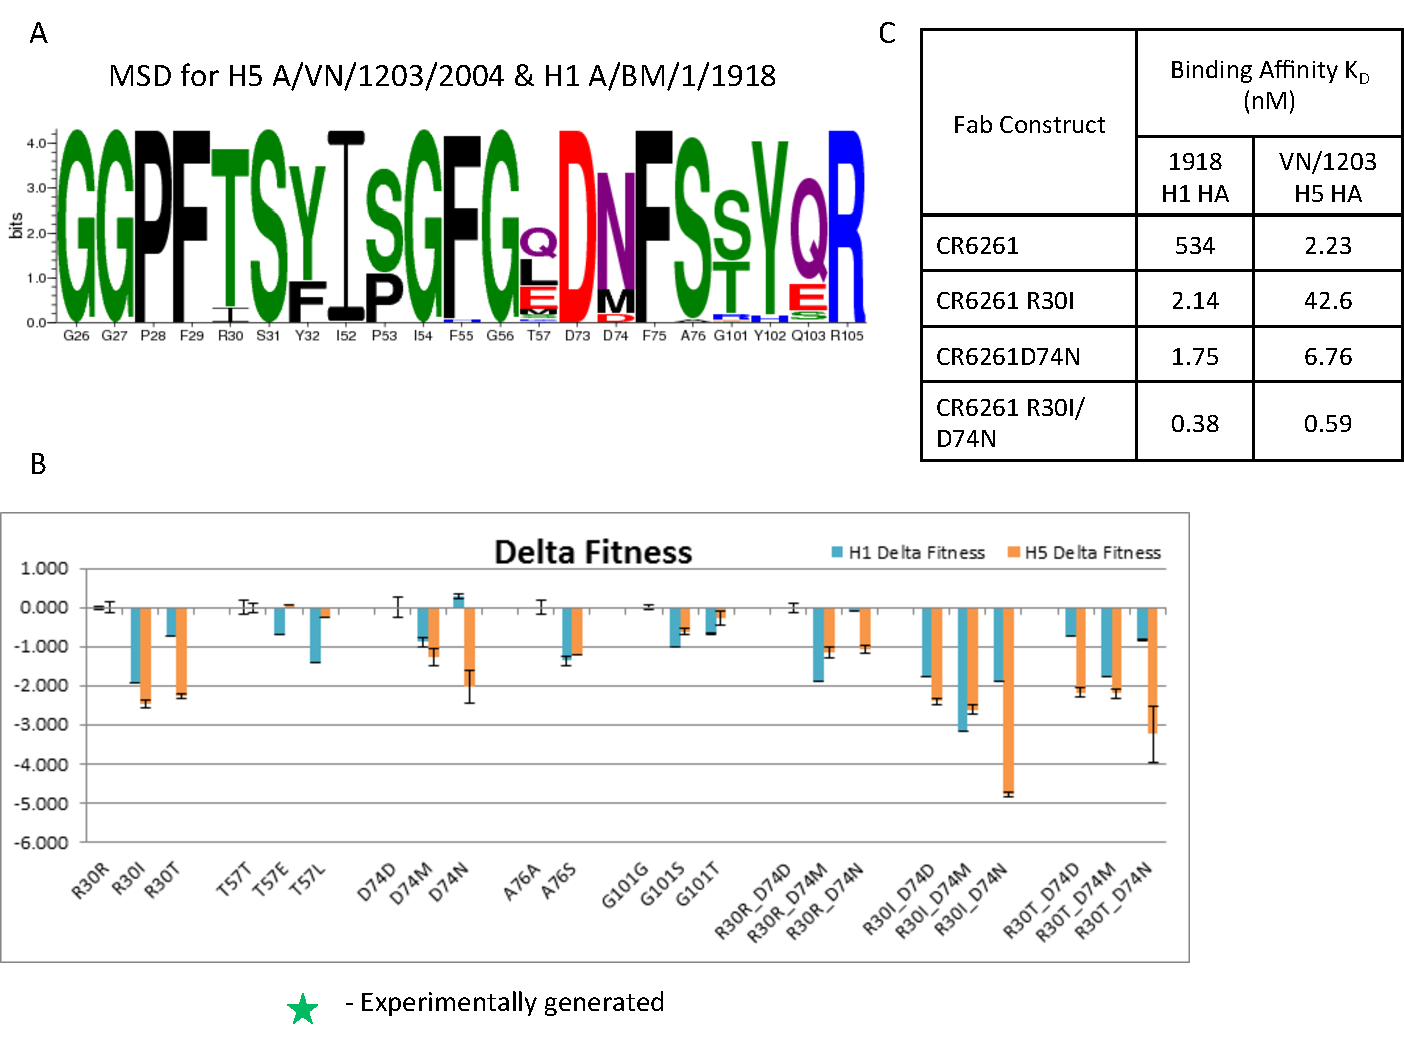
\includegraphics[width=.9\textwidth]{images/chapter5/figure5_2.pdf}
   \caption[Preliminary for MSD Proof-of-Concept]{Preliminary for MSD proof-of-concept. A sequence logo for all positions considered for redesign at the interface. Higher letters indicate \rosetta's proclivity for a certain amino acid sequence (A). Fitness analysis of each position is a sum of stability and binding energy. Lower energies indicate better fitness. Ideally, both H1 and H5 would have decreased fitness energy. Stars indicate mutations that were made experimentally (B). The binding affinities from the suggested mutations from \rosetta. The double mutant gives the best binding affinity (C).}
       \label{fig:fig5_2}
\end{figure}

Of course this mild proof of concept can extend well beyond Influenza. My plan was to use this to get a serotype specific antibody to bind (and therefore, potentially neutralize) cross-serotype, cross-group, and cross Influenza type. However, many groups are trying to design cross specific antibodies. One advantage of multi-state design is that if you fine-tune specificity you do not have to lose specificity to your original epitope. For example, in a paper by Simonelli \textit{et al.} \citep{Simonelli:2013jc}, they used computational modeling along with NMR restraints to place give a molecular definition of an anti-DENV against all four DENV serotypes. They then used their knowledge of rationale design to fine tune specificity to each serotype individually. However, upon making one mutation specific to a given serotype often abrogated binding to the others. Therefore it is possible to enhance breadth at the cost of specificity. This type of problem is ideal for multi-state design as it can fine tune specificity without predicted loss of binding to your original epitope.

In related work, structural viral homologs could also be used in multi-state design. For example, an antibody found in chronically exposed repository infected patients bound and neutralized four different paramyxoviruses, human respiratory syncytial virus (HRSV), human metapneumovirus (HMPV), bovine RSV (BRSV) and pneumonia virus of mice (PVM) \citep{Corti:2013cv}. This antibody was found by screening a common structural homolog (prefusion protein F) against anti-HRSV screened from over 200 donors to narrow down their search. I hypothesize that this type of structural information can be used in multi-state design to make \textit{de novo} designed cross-neutralizers much the way nature selected cross-neutralizers from these patients.

Finally, there is much use for this algorithms fitness function. While I describe antibody design in the context of \textit{designing for} a certain antigen, it may be beneficial to \textit{design against}. I can modify the scoring function in such a way where we select mutations that will \textit{design for} one antigen, and \textit{design against} others. This allows any fine tuning of specificity changes that are needed against antibodies while not compromising the structural integrity of the immunoglobulin fold. I can imagine this will be an invaluable tool for designing against antigens that are found to be related to autoimmunity.

\section{Chapter \ref{chap:chapter3} - Broadly antibodies from HIV-\naive repertoires}


\section{Chapter \ref{chap:chapter4} - Broadly neutralizing antibody redesign}
\section{Other applications of antibody design - antigen escape}